
\documentclass[12pt]{article}
%\usepackage[finnish]{babel}
\usepackage[T1]{fontenc}
\usepackage[utf8]{inputenc}
\usepackage{delarray,amsmath,bbm,epsfig,slashed}
\usepackage{bbold}
\usepackage{listings}
\usepackage{qcircuit}
\newcommand{\pat}{\partial}
\newcommand{\be}{\begin{equation}}
\newcommand{\ee}{\end{equation}}
\newcommand{\bea}{\begin{eqnarray}}
\newcommand{\eea}{\end{eqnarray}}
\newcommand{\abf}{{\bf a}}
\newcommand{\Zmath}{\mathbf{Z}}
\newcommand{\Zcal}{{\cal Z}_{12}}
\newcommand{\zcal}{z_{12}}
\newcommand{\Acal}{{\cal A}}
\newcommand{\Fcal}{{\cal F}}
\newcommand{\Ucal}{{\cal U}}
\newcommand{\Vcal}{{\cal V}}
\newcommand{\Ocal}{{\cal O}}
\newcommand{\Rcal}{{\cal R}}
\newcommand{\Scal}{{\cal S}}
\newcommand{\Lcal}{{\cal L}}
\newcommand{\Hcal}{{\cal H}}
\newcommand{\hsf}{{\sf h}}
\newcommand{\half}{\frac{1}{2}}
\newcommand{\Xbar}{\bar{X}}
\newcommand{\xibar}{\bar{\xi }}
\newcommand{\barh}{\bar{h}}
\newcommand{\Ubar}{\bar{\cal U}}
\newcommand{\Vbar}{\bar{\cal V}}
\newcommand{\Fbar}{\bar{F}}
\newcommand{\zbar}{\bar{z}}
\newcommand{\wbar}{\bar{w}}
\newcommand{\zbarhat}{\hat{\bar{z}}}
\newcommand{\wbarhat}{\hat{\bar{w}}}
\newcommand{\wbartilde}{\tilde{\bar{w}}}
\newcommand{\barone}{\bar{1}}
\newcommand{\bartwo}{\bar{2}}
\newcommand{\nbyn}{N \times N}
\newcommand{\repres}{\leftrightarrow}
\newcommand{\Tr}{{\rm Tr}}
\newcommand{\tr}{{\rm tr}}
\newcommand{\ninfty}{N \rightarrow \infty}
\newcommand{\unitk}{{\bf 1}_k}
\newcommand{\unitm}{{\bf 1}}
\newcommand{\zerom}{{\bf 0}}
\newcommand{\unittwo}{{\bf 1}_2}
\newcommand{\holo}{{\cal U}}
%\newcommand{\bra}{\langle}
%\newcommand{\ket}{\rangle}
\newcommand{\muhat}{\hat{\mu}}
\newcommand{\nuhat}{\hat{\nu}}
\newcommand{\rhat}{\hat{r}}
\newcommand{\phat}{\hat{\phi}}
\newcommand{\that}{\hat{t}}
\newcommand{\shat}{\hat{s}}
\newcommand{\zhat}{\hat{z}}
\newcommand{\what}{\hat{w}}
\newcommand{\sgamma}{\sqrt{\gamma}}
\newcommand{\bfE}{{\bf E}}
\newcommand{\bfB}{{\bf B}}
\newcommand{\bfM}{{\bf M}}
\newcommand{\cl} {\cal l}
\newcommand{\ctilde}{\tilde{\chi}}
\newcommand{\ttilde}{\tilde{t}}
\newcommand{\ptilde}{\tilde{\phi}}
\newcommand{\utilde}{\tilde{u}}
\newcommand{\vtilde}{\tilde{v}}
\newcommand{\wtilde}{\tilde{w}}
\newcommand{\ztilde}{\tilde{z}}

% David Weir's macros


\newcommand{\nn}{\nonumber}
\newcommand{\com}[2]{\left[{#1},{#2}\right]}
\newcommand{\mrm}[1] {{\mathrm{#1}}}
\newcommand{\mbf}[1] {{\mathbf{#1}}}
\newcommand{\ave}[1]{\left\langle{#1}\right\rangle}
\newcommand{\halft}{{\textstyle \frac{1}{2}}}
\newcommand{\ie}{{\it i.e.\ }}
\newcommand{\eg}{{\it e.g.\ }}
\newcommand{\cf}{{\it cf.\ }}
\newcommand{\etal}{{\it et al.}}
\newcommand{\ket}[1]{\vert{#1}\rangle}
\newcommand{\bra}[1]{\langle{#1}\vert}
\newcommand{\bs}[1]{\boldsymbol{#1}}
\newcommand{\xv}{{\bs{x}}}
\newcommand{\yv}{{\bs{y}}}
\newcommand{\pv}{{\bs{p}}}
\newcommand{\kv}{{\bs{k}}}
\newcommand{\qv}{{\bs{q}}}
\newcommand{\bv}{{\bs{b}}}
\newcommand{\ev}{{\bs{e}}}
\newcommand{\gv}{\bs{\gamma}}
\newcommand{\lv}{{\bs{\ell}}}
\newcommand{\nabv}{{\bs{\nabla}}}
\newcommand{\sigv}{{\bs{\sigma}}}
\newcommand{\notvec}{\bs{0}_\perp}
\newcommand{\inv}[1]{\frac{1}{#1}}
%\newcommand{\xv}{{\bs{x}}}
%\newcommand{\yv}{{\bs{y}}}
\newcommand{\Av}{\bs{A}}
%\newcommand{\lv}{{\bs{\ell}}}
\newcommand{\Rmath}{\mbf{R}}


%\newcommand\bsigma{\vec{\sigma}}
\hoffset 0.5cm
\voffset -0.4cm
\evensidemargin -0.2in
\oddsidemargin -0.2in
\topmargin -0.2in
\textwidth 6.3in
\textheight 8.4in

\begin{document}

\normalsize

\baselineskip 14pt

\begin{center}
{\Large {\bf Quantum Information B \ \ Fall 2020 \ \  Solutions to Problem Set 1}} \\
Jake Muff \\
1/11/20
\end{center}

\bigskip
\section{Answers}



\begin{enumerate}
    \item Exercise 6.3 Nielsen and Chaung. Show that in the $\ket{\alpha}, \ket{\beta}$ basis we can write the Grover iteration as 
    $$ G = \left(\begin{array}{cc} \cos(\theta) & -\sin(\theta) \\  \sin(\theta) & \cos(\theta) \end{array}\right)$$
    The grover iteration is written as 
    $$ H^{\otimes n} P H^{\otimes n} = 2 \ket{\psi}\bra{\psi}-I $$
    And the Oracle $O$
    $$ O = I - 2 \ket{\beta}\bra{\beta} $$
    So that 
    $$ G = O \cdot H^{\otimes n} P H^{\otimes n} $$ 
    $$ G = (I - 2\ket{\beta}\bra{\beta})(2\ket{\psi}\bra{\psi}-I) $$
    $$ = 2\ket{\psi}\bra{\psi} - I - 4\ket{\beta}\bra{\beta}\ket{\psi}\bra{\psi} + 2\ket{\beta}\bra{\beta} $$
    We take the case where $M=1$ so that 
    $$ \ket{\psi} = \sqrt{1-\frac{1}{N}}\ket{\alpha}+ \sqrt{\frac{1}{N}}\ket{\beta} $$
    Using the fact that $I = \ket{\alpha}\bra{\alpha}+\ket{\beta}\bra{\beta}$ 
    $$ G = 2 \Big[ \frac{1}{N} \ket{\beta}\bra{\beta}+ \frac{\sqrt{N-1}}{N}(\ket{\beta}\bra{\alpha}+\ket{\alpha}\bra{\beta})+ \frac{N-1}{N} \ket{\alpha}\bra{\alpha} \Big] $$
    $$ - \ket{\beta}\bra{\beta}- \ket{\alpha}\bra{\alpha} - 4 \ket{\beta} \Big(\sqrt{\frac{1}{N}}\Big)\Big( \sqrt{\frac{1}{N}}\bra{\beta}+\sqrt{\frac{N-1}{N}} \bra{\alpha} \Big) + 2 \ket{\beta}\bra{\beta} $$
    $$ G = (1- \frac{2}{N})(\ket{\beta}\bra{\beta} + \ket{\alpha}\bra{\alpha}) + \frac{2 \sqrt{N-1}}{N}(\ket{\alpha}\bra{\beta}-\ket{\beta}\bra{\alpha}) $$
    If we have $\cos(\theta) = (1-\frac{2}{N})$ then $\sin(\theta) = \sqrt{1-\cos(\theta)} = \frac{2 \sqrt{N-1}}{N} $, then $G$ is 
    $$ G = \cos(\theta)(\ket{\beta}\bra{\beta} + \ket{\beta}\bra{\beta}) + \sin(\theta)(\ket{\alpha}\bra{\beta}-\ket{\beta}\bra{\alpha}) $$
    And we have 
    $$ G = \left(\begin{array}{cc} \cos(\theta) & -\sin(\theta) \\  \sin(\theta) & \cos(\theta) \end{array}\right)$$

    \item Exercise 6.5. Show that the augmented oracle $O'$ may be constructed using one application of $O$ and elementary quantum gates using the extra quibt $\ket{q}$. The augmented oracle only marks an item if it is a solution and the extra qubit is set to 0. Equation 6.1 from the book tells us that $\ket{q}$ is flipped if $f(x) =1$ and unchanged otherwise. Much like in Fig 4.11 in the book where an X gate was used we can use the Pauli $Z$ gate as we wanted to leave the qubit in state $\ket{0}$ unchanged and sign flip if the state is $\ket{1}$. 
    \\
    The application of the normal oracle is 

    \begin{figure}[h]
        
        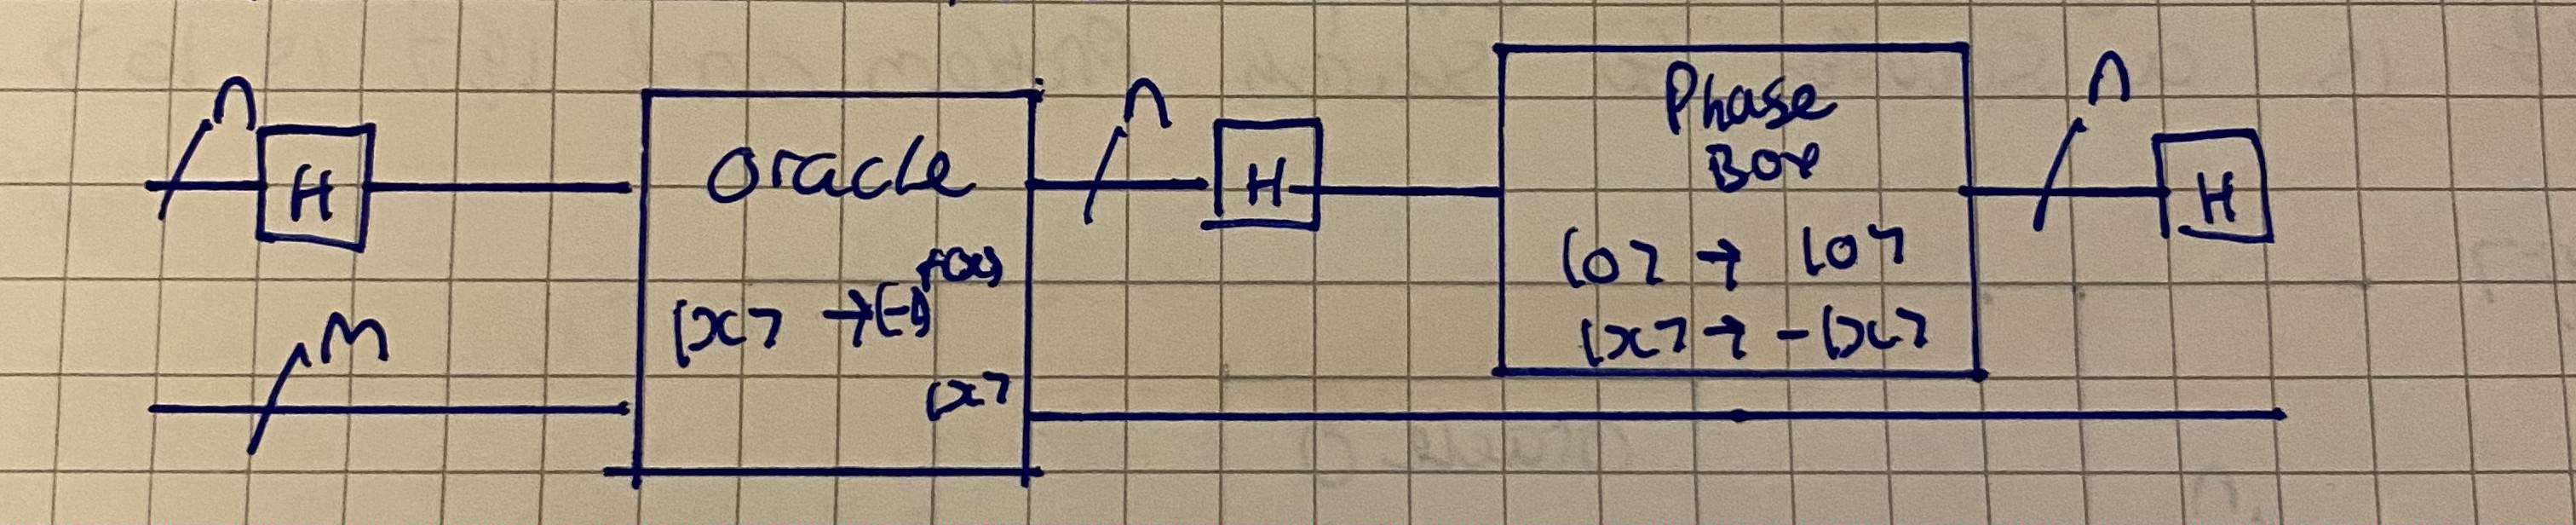
\includegraphics[width=10cm]{Oracle.jpg}
        \centering
        \caption{Circuit implementing the Oracle $O$}
    \end{figure}
    The circuit for the augmented oracle $O'$. $\frac{\ket{0} - \ket{1}}{2}$ is the initial state. $\backslash n$ represents $n$ wires. 
    \begin{figure}[h]
        
        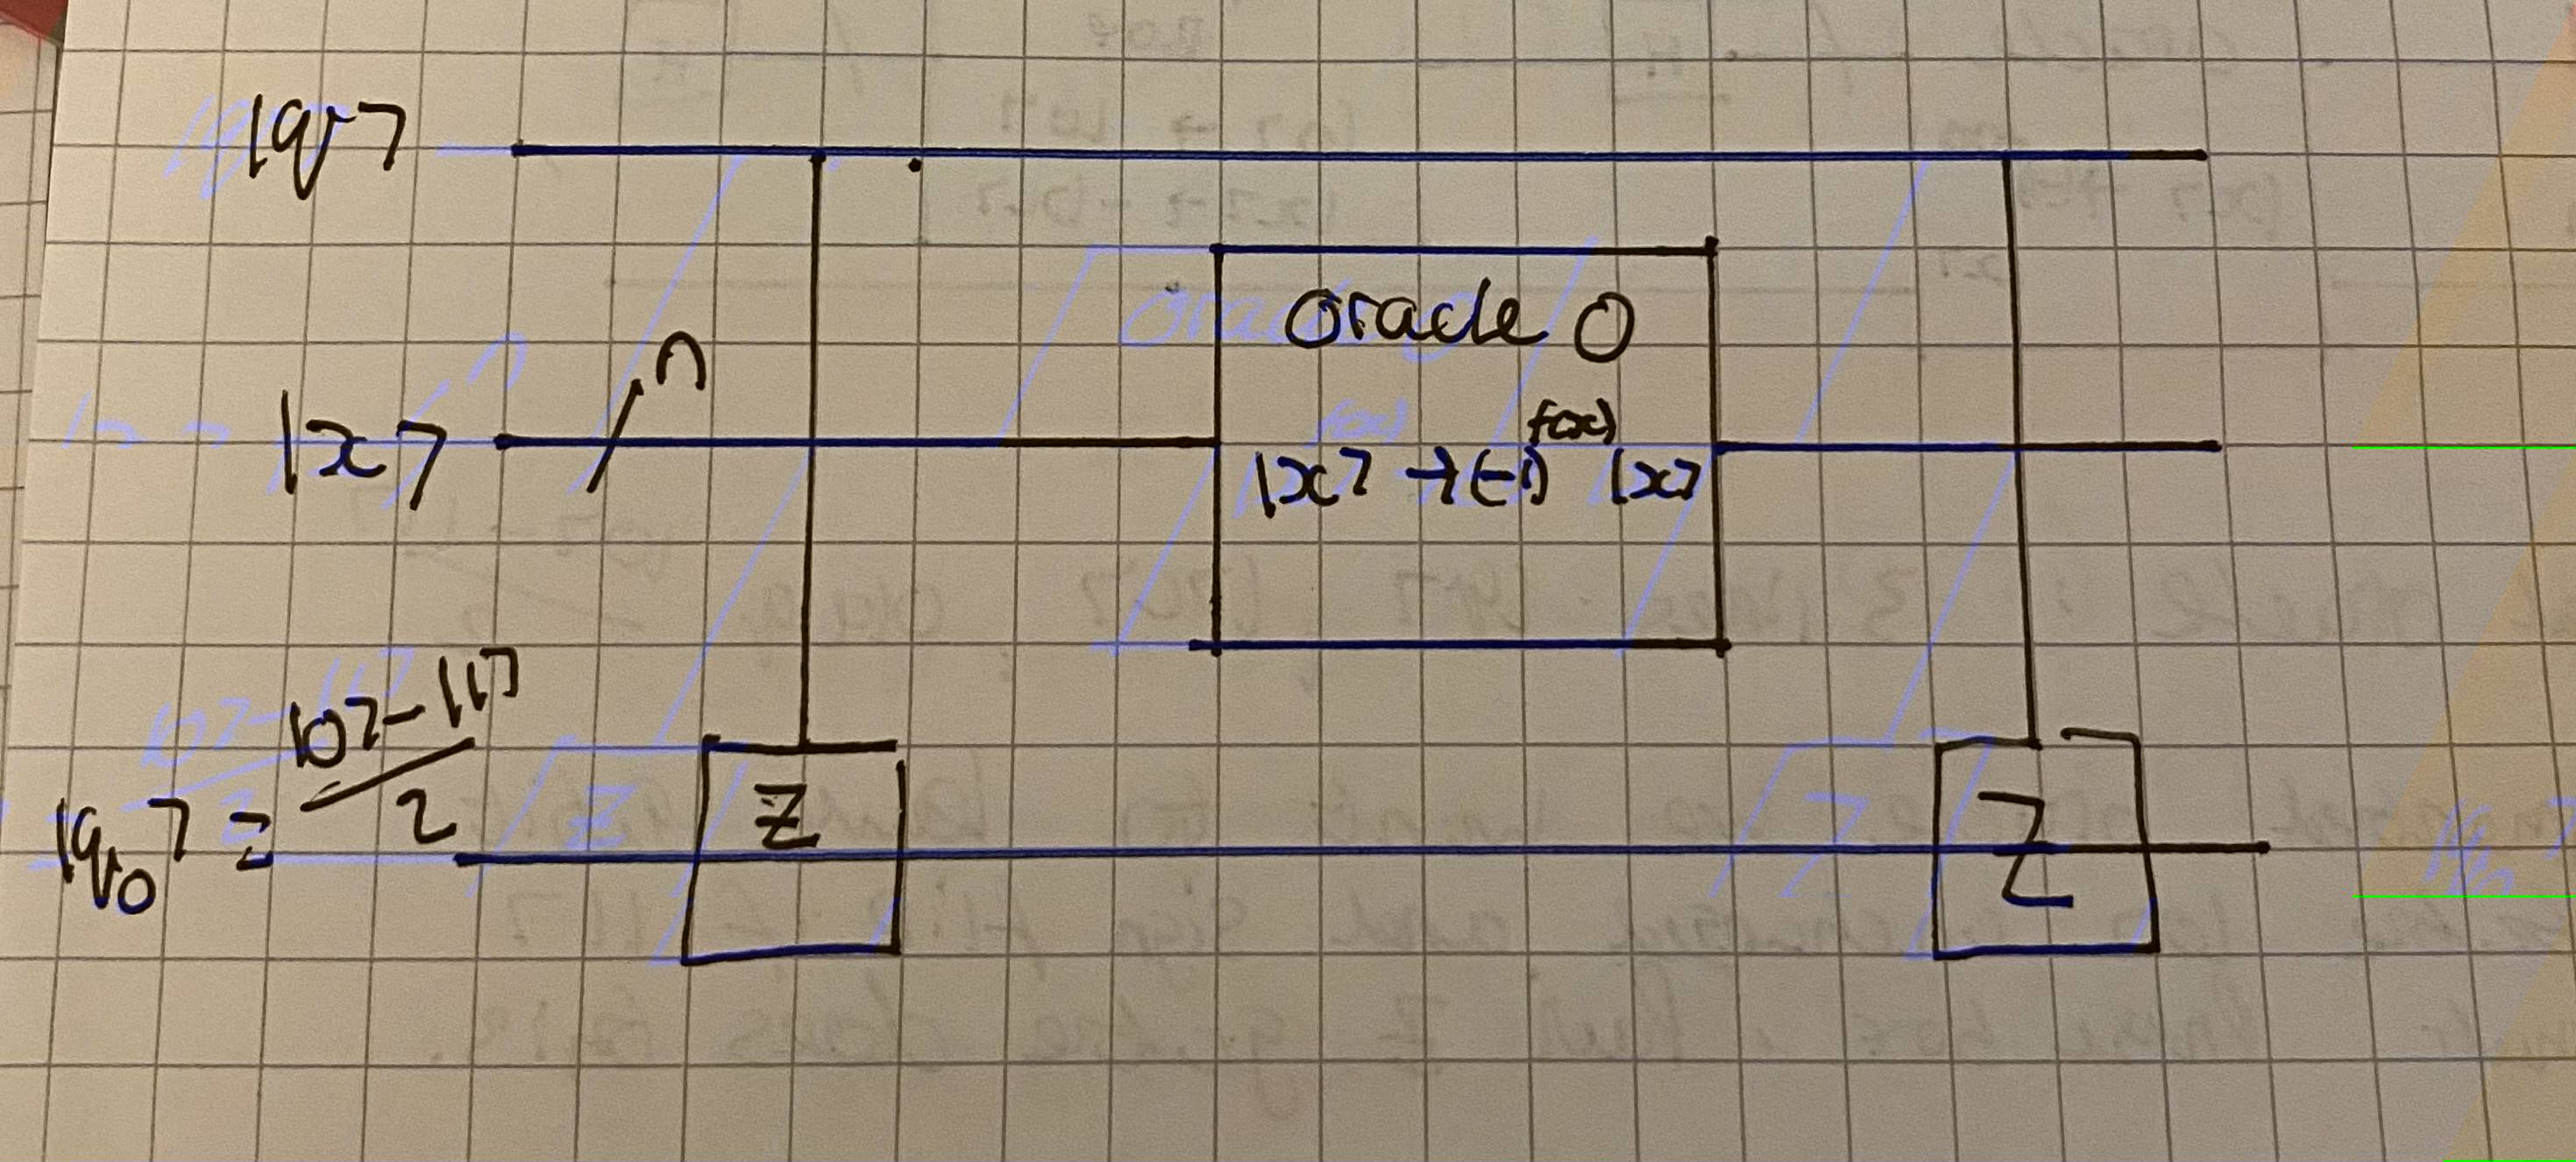
\includegraphics[width=10cm]{Augmented Oracle.jpg}
        \centering
        \caption{Circuit implementing the Augmented Oracle $O'$}
    \end{figure}

    \item Exercise 6.6. Verify that the gates in the dotted box in the second figure of box 6.1 perform the conditional phase shift operation $2 \ket{00} \bra{00} - I$ up to an umimportant phase factor. 
    \\
    \begin{figure}[h]
        
        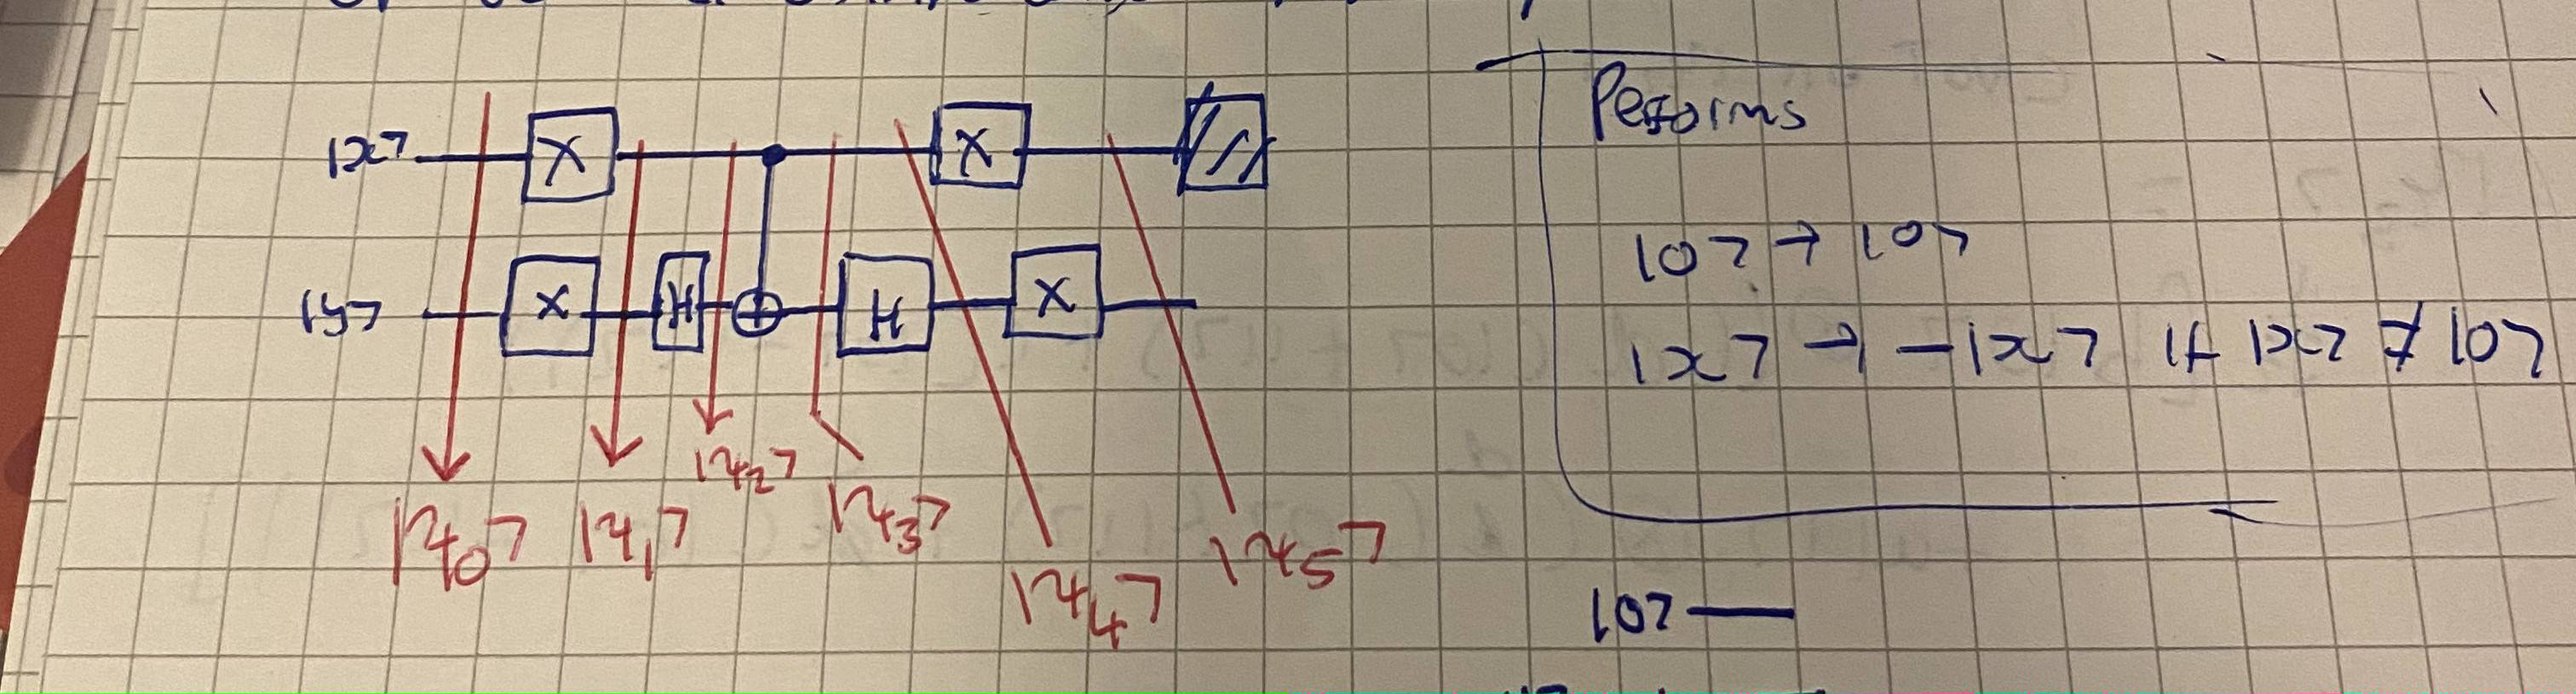
\includegraphics[width=10cm]{Phasecircuit.jpg}
        \centering
        \caption{Circuit from dotted box in second figure of Box 6.1. The red lines are where we calculate the state}

    \end{figure}
    %We have 
    $$ \ket{x} = \ket{0}^{\otimes n} \ket{0}^{\otimes n} \rightarrow a \ket{0} + b \ket{1} $$
    $$ \ket{y} = \ket{0}^{\otimes n} \ket{1} \rightarrow c \ket{0} + d \ket{1} $$
    The initial state is 
    $$ \ket{\psi_0} =(\ket{0} \otimes \ket{0})(\ket{0} \otimes \ket{1}) $$
    $$ = (a \ket{0} + b\ket{1})( c \ket{0} + d\ket{1}) $$
    After the $X$ gates 
    $$ \ket{\psi_1} = X(a \ket{0} + b \ket{1}) X (c \ket{0} + d \ket{1}) $$
    $$ = (b \ket{0} + a \ket{1})(d \ket{0} + c \ket{1}) $$
    After the $H$ gate 
    $$ \ket{\psi_2} = ( b\ket{0} + a\ket{1})H(d \ket{0} + c\ket{1}) $$
    $$ =(b \ket{0} + a \ket{1})\Big( d \frac{\ket{0} + \ket{1}}{\sqrt{2}} + c \frac{\ket{0} - \ket{1}}{\sqrt{2}}\Big)$$
    $$ = \frac{1}{\sqrt{2}} (b \ket{0} + a \ket{1})(c (\ket{0} + \ket{1}) + d(\ket{0} - \ket{1})) $$
    Apply the CNOT to $\ket{\psi_2}$ 
    $$ \ket{\psi_3} = \frac{1}{\sqrt{2}} \Big[ b \ket{0} \otimes \Big( d (\ket{0} + \ket{1}) + c(\ket{0} - \ket{1}) \Big) + a \ket{1} \otimes \Big( d(\ket{0} + \ket{1}) + c(\ket{0} - \ket{1}) \Big) \Big]$$
    $$ = \frac{1}{\sqrt{2}} \Big[ b \ket{0} \big( ( d+c)\ket{0} + (d-c)\ket{1} \big) + a \ket{1} \big( (d+c)\ket{0} + (d-c) \ket{1} \big) \Big] $$
    After the second $H$ gate
    $$ \ket{\psi_4} = b \ket{0} ( d \ket{0} + c \ket{1}) + a \ket{1} ( d\ket{0} - c \ket{1}) $$
    And the final state is 
    $$ \ket{\psi_5} = a \ket{0} (-c \ket{0} + d \ket{1}) + b\ket{1}(c \ket{0} + d \ket{1})$$
    Expanding 
    $$ = -a c \ket{00} + ad \ket{01} + bc \ket{10} + bd \ket{11}) $$
    For this to perform the quantum search we have $\ket{x} \rightarrow - \ket{x}$ or in this case $\ket{00} \rightarrow - \ket{00} $. So $\ket{\psi_5}$ can be written as 
    $$ -2 \ket{00} \bra{00} + I $$ 
    Or 
    $$ -(2 \ket{00} \bra{00} - I)  $$
    $$ = -( 2 \ket{00} - I) \ket{xy} $$
    Where $-$ is the unimportant phase factor. 

    \item Exericse 6.9. Verify 
    $$ U (\Delta t) = \Big( \cos^2(\frac{\Delta t}{2}) - \sin^2(\frac{\Delta t}{2}) \vec{\psi} \cdot \hat{z} \Big) I $$
    $$ - 2i \sin(\frac{\Delta t}{2})\Big( \cos(\frac{\Delta t}{2}) \frac{\vec{\psi}+\hat{z}}{2} + \sin(\frac{\Delta t}{2}) \frac{\vec{\psi} \times \hat{z}}{2} \Big) $$
    From the book we know that 
    %\frac{\Delta t}{2}
    $$ U(\Delta t) \equiv \exp(-i \ket{\psi}\bra{\psi} \Delta t) \exp(-i \ket{x}\bra{x} \Delta t) $$
    From Chapter 4 (eq 4.8) we know that 
    $$ \exp(i Ax) = cos(x) I + isin(x)A $$ 
    So we have 
    $$ R_{\vec{\psi}} = \exp(-i \ket{\psi}\bra{\psi} \Delta t) $$
    $$ = \cos(\frac{\Delta t}{2})I -i \sin(\frac{\Delta t}{2})(\vec{\psi} \cdot \vec{\sigma}) $$
    $$ R_{\hat{z}} =  \exp(-i \ket{x}\bra{x} \Delta t) $$
    $$ = \cos(\frac{\Delta t}{2}) - i \sin(\frac{\Delta t}{2}) (\hat{z} \cdot \vec{\sigma}) $$
    And 
    $$ U(\Delta t) = R_{\vec{\psi}} R_{\hat{z}} $$
    $$ U(\Delta t) = \Big[ \cos(\frac{\Delta t}{2}) -isin(\frac{\Delta t}{2})(\vec{\psi} \cdot \vec{\sigma}) \Big] \cdot \Big[ \cos(\frac{\Delta t}{2}) -isin(\frac{\Delta t}{2})(\hat{z} \cdot \vec{\sigma}) \Big] $$
    $$ = \cos(\frac{\Delta t}{2}) \cos(\frac{\Delta t}{2})I - \sin(\frac{\Delta t}{2}) \sin(\frac{\Delta t}{2})(\vec{\psi} \cdot \vec{\sigma})(\hat{z} \cdot \vec{\sigma}) $$ 
    $$ -i \sin(\frac{\Delta t}{2}) \cos(\frac{\Delta t}{2})(\hat{z} \cdot \vec{\sigma}) -i \cos(\frac{\Delta t}{2}) \sin(\frac{\Delta t}{2}) (\vec{\psi} \cdot \vec{\sigma}) $$
    Introducing an identity (From Ex 4.15)
    $$ (\vec{\psi} \cdot \vec{\sigma})(\hat{z} \cdot \vec{\sigma}) = \hat{z} \cdot \vec{\psi}I + i(\vec{\psi} \times \hat{z}) \cdot \vec{\sigma} $$
    Implementing and simplifying 
    $$ R_{\vec{\psi}} R_{\hat{z}}  = $$
    $$ \cos^2 (\frac{\Delta t}{2})I - \sin^2(\frac{\Delta t}{2}) \Big[ \hat{z} \cdot \vec{\psi} + i(\vec{\psi} \times \hat{z}) \cdot \vec{\sigma} \Big] \ldots $$
    $$ -i \sin(\frac{\Delta t}{2}) \cos(\frac{\Delta t}{2})(\hat{z} \cdot \vec{\sigma}) -i \cos(\frac{\Delta t}{2}) \sin(\frac{\Delta t}{2}) (\vec{\psi} \cdot \vec{\sigma}) $$
    Take out $i$ from the second part 
    $$ =  \cos^2 (\frac{\Delta t}{2}) - \sin^2(\frac{\Delta t}{2})(\vec{\psi} \cdot \hat{z})I \ldots $$
    $$ -i \Big(\sin(\frac{\Delta t}{2}) \cos(\frac{\Delta t}{2}) \hat{z} + \cos(\frac{\Delta t}{2}) \sin(\frac{\Delta t}{2}) \vec{\psi} + \sin(\frac{\Delta t}{2}) \sin(\frac{\Delta t}{2}) (\vec{\psi} \times \hat{z}) \Big) \cdot \vec{\sigma}$$
    Take out $\sin(\frac{\Delta t}{2})$ from the second part 
    $$ = \cos^2(\frac{\Delta t}{2}) - \sin^2(\frac{\Delta t}{2}) (\vec{\psi} \cdot \hat{z})I \ldots $$
    $$ -i \sin(\frac{\Delta t}{2}) \Big( \cos(\frac{\Delta t}{2}) \hat{z} + \cos(\frac{\Delta t}{2}) \vec{\psi} + \sin(\frac{\Delta t}{2}) (\vec{\psi} \times \hat{z}) \Big) \cdot \vec{\sigma} $$
    Take out a factor of 2 
    $$ = \cos^2(\frac{\Delta t}{2}) - \sin^2(\frac{\Delta t}{2}) (\vec{\psi} \cdot \hat{z})I \ldots $$
    $$ -2i \sin(\frac{\Delta t}{2}) \Big( \frac{\cos(\frac{\Delta t}{2})}{2} \hat{z} + \frac{\cos(\frac{\Delta t}{2})}{2}\vec{\psi} + \frac{\sin(\frac{\Delta t}{2})}{2} (\vec{\psi} \times \hat{z}) \Big) \cdot \vec{\sigma} $$
    Which collating terms gives us 
    $$ = \cos^2(\frac{\Delta t}{2}) - \sin^2(\frac{\Delta t}{2}) (\vec{\psi} \cdot \hat{z})I - 2i \sin(\frac{\Delta t}{2}) \Big( \cos(\frac{\Delta t}{2}) (\frac{\hat{z} + \vec{\psi}}{2} ) + \sin(\frac{\Delta t}{2}) (\frac{\vec{\psi} \times \hat{z}}{2}) \Big) \cdot \vec{\sigma} $$
    And clearly this is equal to the equation in the book. 
    \item Problem 6.2 not attempted. 


\end{enumerate}


\end{document}

